
\section{Alimentação} % (fold)
\label{sec:alimentação}
	
	O sistema de alimentação pode ser dividido em 2 grandes grupos: \textit{Bateria} e \textit{Carregador}, os quais estão descritos nas sub-seções dispostas a seguir.

	\subsection{Bateria de íon-lítio (Li-Ion)} % (fold)
	\label{sub:bateria}
		
		De todos os tipos de baterias esta é, sem dúvida, a melhor. Suas vantagens são diversas e variadas e não é justamente por isso que elas são empregadas em larga escala nos novos eletrônicos.

		Não-tóxicas, com capacidade de carga duas vezes maior que as de Ni-MH e três vezes maior que as de NiCd, sem efeito memória (ou seja, a bateria não vai “viciar”) e também mais leves, afinal o lítio é um dos metais mais leves já conhecidos. A densidade do lítio também permite a criação de baterias com maior capacidade.

		Outro ponto que dá muito mais vantagens às baterias de Li-Ion é o fato de estas baterias dispensarem ciclos completos de cargas, ou seja, não é necessário esperar a carga acabar para carregá-la novamente e quando carrega não precisa esperar que ela seja preenchida por completo. Além disso, ao estar carregada por completo a bateria cessa automaticamente o recebimento de energia para evitar sobrecargas.

		Estas baterias, porém, demandam um cuidado maior por parte de seus usuários, como por exemplo, a não exposição a altas temperaturas que podem causar danos definitivos e até mesmo sua explosão.

	\subsubsection{Bateria utilizada}

		A 18650 é uma bateria de 4.2V e possui 8.8Ah. É de Li-íon assim como as baterias de celular, no entanto possuindo maior capacidade energética. A figura \ref{img:bateria} mostra a bateria NK 18650.

		\begin{figure}[H]
			\centering
			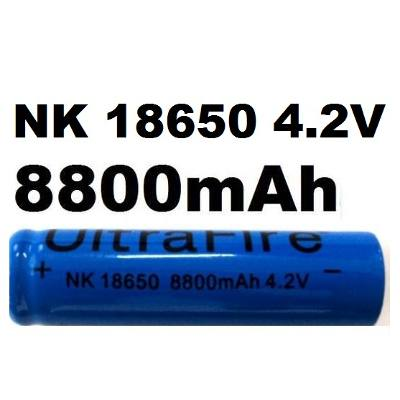
\includegraphics[scale=0.7]{figuras/bateria.jpg}
			\caption{Bateria NK 18650 Ultrafire.}
			\label{img:bateria}
		\end{figure}

		O Li-ion tem melhor relação de peso e potência que as baterias de Ni-MH ou Ni-Cd, tendo apenas o problema da tensão ser mais elevada.

		Usando o princípio da associação de fontes de tensão, resultará em um somatório das tensões das fontes. Quando 3 baterias de 4.2V são associadas em série temos o equivalente a um bateria de 12.6V, internamente em uma bateria é possível distinguir 3 células de 4.2V. Mas é preciso atentar que para resultar neste somatório todas as células ou fontes tem de estar com as polaridades sempre entre positivo para negativo ou vice versa.

	\subsubsection{Consumo energético}

		Foi realizada uma relação de consumo e capacidade de energia dos componentes para a escolha da bateria ideal, onde os motores consomem a maior parte da corrente.

		\begin{table}[H]
		\centering
		\caption{Consumo energético.}
		\label{tab:consumo_energético}
		\begin{tabular}{lllll}
		Componente               & Quantidade & Corrente unitária (mA) & Corrente total (mA) & Tensão (V) \\ \hline
		Ponte H                & 1          & 36                     & 36                  & 6          \\ \hline
		AtMega                 & 1          & 500                    & 500                 & 5          \\ \hline
		Motor DC               & 3          & 470                    & 1410                & 6          \\ \hline
		Módulo ESP8266         & 1          & 1000                   & 1000                & 3.3        \\ \hline
		Motor DC \\ 12V Aspiração & 1           & 4400                   & 4400                & 12         \\ \hline
		TOTAL                  &            &                        & 7421                & \\ \hline          
		\end{tabular}
		\end{table}

		De acordo com a tabela \ref{tab:consumo_energético}, é possível analisar a corrente e tensão de cada componente utilizado no projeto. Os componentes utilizados trabalharão com uma média de 7Ah, sendo que, um dos requisitos do robô é ter de aspirar um cômodo de maneira autônoma durante 30 minutos, com isto a corrente diminui para 3.5Ah.


	% subsection bateria (end)

	\subsection{Carregador} % (fold)
	\label{sub:carregador}
	
		Uma das grandes dificuldades na aplicação do sistema de alimentação em um projeto de eletrônico portátil é a forma com que se vai fornecer os ciclos de carga ao aparelho. No que tange as especificidades do projeto, por ser um aspirador de pó que opera de forma autônoma, o maior desafio foi encontrar uma maneira de fazer com que o robô, após notar a necessidade, se dirigisse a sua base e começasse a se recarregar da forma mais simples e prática possível. 

Depois de diversas pesquisas e muitas hipóteses consideradas, chegou-se em consenso de que o princípio de carregamento por indução eletromagnética é o que se adequa ao projeto, já que não é necessário a conexão de cabos/conectores.

A indução eletromagnética consiste basicamente no surgimento de uma corrente elétrica oriunda de um fluxo magnético próximo de um condutor. O conceito é antigo e teve o princípio do raciocínio em 1820, quando Hans Christian Oesterd descobriu que cargas elétricas em movimento davam origem a um campo magnético.

 Tal descoberta levou diversos estudiosos da época a creer que o inverso também deveria ser possível de acontecer, ou seja: a varição do campo magnético levaria a uma produção de corrente elétrica. Michael Faraday, também dinamarquês, em 1931, batizou esse comportamento como indução eletromagnética e comprovou tal teoria através daquela que é conhecida até hoje com a Lei de Faraday.

 \begin{figure}[H]
	\centering
	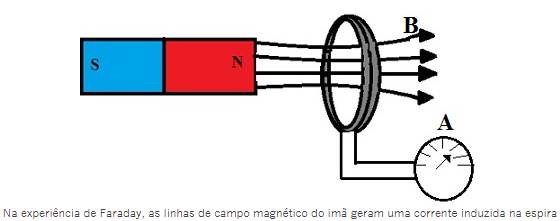
\includegraphics[scale=0.7]{figuras/carregador_inducao}
	\caption{Experiência de Faraday.}
	\label{img:faraday}
\end{figure}

A Lei de Faraday diz que uma força eletromotriz é produzida por condutores elétricos que se movimentam num campo magnético uniforme, ou então por um campo magnético variável. Tem uma melhor exemplificação da seguinte forma:


	$Fem = \frac{-d \phi }{dt}$


Sendo Fem a força eletromotriz (V), $\phi$ o fluxo magnético e t o tempo. Algum tempo depois James Clerk Maxwell, analisando o experimento de Faraday, escreveu uma outra lei que relaciona os campos elétrico e magnético, como podemos ver abaixo:


	$\nabla xE = \frac{-dB}{dt}$


Sendo $\nabla$ o operador nabla, E o campo elétrico e B o campo magnético. Analisando essa formulação conclui-se que o rotacional do campo elétrico é igual ao oposto da variação do campo magnético no tempo.


Esse conceito já é frequentemente utilizado em transformadores elétricos, motores, máquinas de indução em geral que hoje também englobam os carregadores mais modernos, afim de fornecer correntes de carga para baterias, especialmente para aparelhos como notebooks, tablets, smartphones e  e etc.

 \begin{figure}[H]
	\centering
	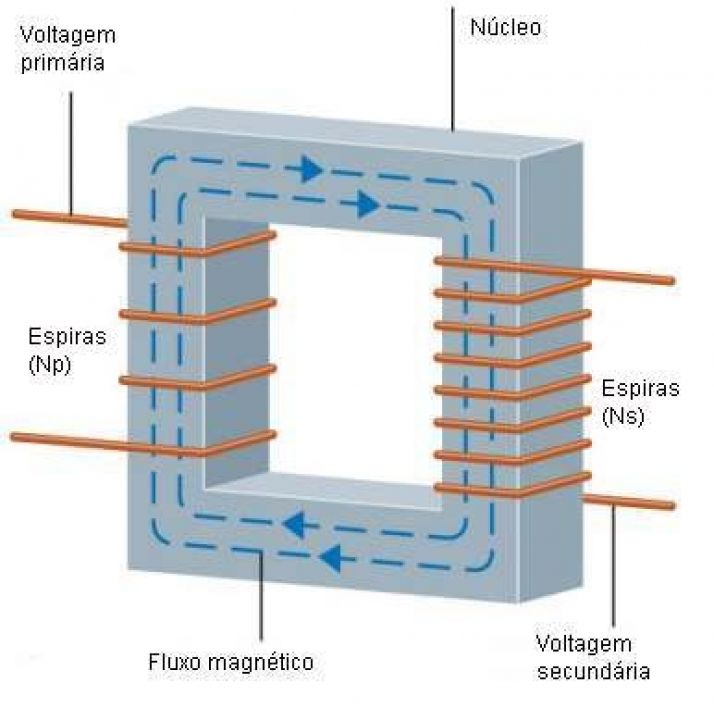
\includegraphics[scale=0.5]{figuras/transformador}
	\caption{Transformador elétrico.}
	\label{img:transformador}
\end{figure}

 \begin{figure}[H]
	\centering
	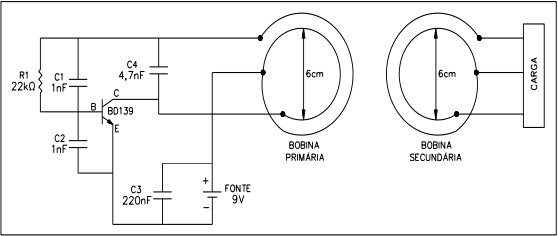
\includegraphics[scale=0.5]{figuras/diagrama_eletrico}
	\caption{Diagrama elétrico.}
	\label{img:diagrama_eletrico}
\end{figure}

A função do circuito da figura \ref{img:diagrama_eletrico} é transformar \textit{direct current} - DC em \textit{alternating current} – AC. Sabe-se que para carregar as baterias o sistema deve fornecer uma corrente contínua, para isso utilizou-se uma ponte de diodo entre a conexão da bobina secundária e o elemento que se desejou alimentar.
Os primeiros testes foram realizados na estrutura supracitada, que representa o protótipo de um carregador por indução. Para isso foram utilizados três capacitores, um resistor, um transistor, vários indutores (bobinas).
Os testes realizados objetivaram observar o comportamento das perdas na primeira parcela e verificar a tensão e corrente entregues na segunda parcela do sistema a fim verificar a eficiência e a viabilidade do modelo pré-estabelecido.
As tabelas \ref{tab:resultadotestescarregadorinducao} e \ref{tab:resultadotestescarregadorinducao2} expõe os resultados obtidos.

\begin{table}[]
\centering
\caption{Resultados do teste 1.}
\label{tab:resultadotestescarregadorinducao}
\begin{tabular}{l|l|l|l|}
\cline{2-4}
\textbf{}                                        & \textbf{Nº de espiras} & \textbf{Tensão (v)} & \textbf{Corrente (mA)} \\ \hline
\multicolumn{1}{|l|}{\textbf{Bobina 1 (6 mm)}}   & 6                      & 9.8                 & -                      \\ \hline
\multicolumn{1}{|l|}{\textbf{Bobina 2 (0.6 mm)}} & 20                     & 6.2                 & 0.7                    \\ \hline
\end{tabular}
\end{table}

\begin{table}[]
\centering
\caption{Resultados do teste 2.}
\label{tab:resultadotestescarregadorinducao2}
\begin{tabular}{l|l|l|l|}
\cline{2-4}
\textbf{}                                        & \textbf{Nº de espiras} & \textbf{Tensão (v)} & \textbf{Corrente (mA)} \\ \hline
\multicolumn{1}{|l|}{\textbf{Bobina 1 (0.6 mm)}} & 20                     & 5.6                 & -                      \\ \hline
\multicolumn{1}{|l|}{\textbf{Bobina 2 (0.6 mm)}} & 20                     & 2.62                & 2.2                    \\ \hline
\end{tabular}
\end{table}

Nos testes iniciais foi possível analisar o desempenho do sistema para que as devidas alterações pudessem ser feitas. 
Identificou-se que a bobina secundária deveria estar posicionada no inferior da estrutura da base do robô, visto que esta, devido ao material que a compõe, interfere de forma prejudicial ao fluxo que chega à segunda bobina. Além da necessidade de se aumentar a tensão e a corrente a serem entregues pela ponte de diodo, pois necessitamos de uma tensão de 14.8V e uma corrente de 2A para alimentar a bateria.
De fato pode-se constatar que a corrente obtida a partir dos testes realizados não é suficiente para realizar a recarga das baterias. Uma busca por novas alternativas para aumentar os parâmetros contínuos de saída na bobina secundária ainda estão sendo implementadas. De forma paralela uma nova solução, carregador com plug magnético, está sendo desenvolvida.

Algumas alterações nos componentes do circuito se fizeram necessárias para se iniciar a segunda fase de testes, como: a substituição do transistor P2N2 por um transistor de potência IRF04A a fim de aumentar a capacidade do circuito, além da troca da resistência, na tentativa de atingir os valores necessários para a carga da bateria.
Os testes efetuados na etapa dois tinham como objetivo, verificar a corrente e a tensão alternadas na bobina primária e os valores de tensão e corrente contínua que estavam sendo entregues pela ponte de diodo. Verificou-se experimentalmente que só a troca dos componentes não bastou para constatação desses valores, pois utilizamos uma protoboard que limitava a corrente em 1A, desta forma verificamos que a estrutura mais adequada para realização de testes futuros seria uma placa impressa feita especialmente para o nosso circuito.
Descartamos a possibilidade de carregar as baterias com o carregador por indução, pois mesmo que conseguíssemos alcançar o valor da tensão desejada seria um desafio entregar a corrente solicitada pela bateria, além de que levando em consideração os testes realizados na primeira etapa, constatou-se que a corrente que deveria ser entregue para bateria deve ser 500 vezes maior do que a corrente entregue pelo primeiro protótipo.
Concluiu-se que o carregador com plug magnético é a melhor solução para o carregamento da bateria, porém os testes com o carregador por indução irão permanecer a fim de se atingir melhorias do sistema e possíveis resultados para atividades futuras do \textit{R2-PI2}.

\subsection{Carregador com plug magnético}

Este carregador deverá ser capaz de fornecer uma tensão próxima de 16V e corrente de 2A, sendo que o mesmo foi feito para garantir o carregamento das baterias já que existe o risco de que o carregador por indução não entregue a tensão necessária
A tensão fornecida pela concessionária de energia elétrica é alternada ao passo que os dispositivos eletrônicos operam em tensão contínua. Então é necessário retificá-la e isto é feito por meio de circuitos retificadores que convertem corrente alternada em corrente contínua. Temos os retificadores monofásicos para uso em aparelhos eletrônicos de um modo geral e os retificadores polifásicos para uso em circuitos industriais de alta potência. 
No circuito deste carregador é utilizado um retificador em ponte, um circuito elétrico com o objetivo de converter as tensões de alternadas para contínuas, por meio de um processo de conversão de elementos semicondutores, tais como a conexão com pontes de diodo, dispositivos eletrônicos feitos de silício ou germânio capazes de converter ac em dc. A corrente fornecida pela tomada é alternada, ou seja, mudam sua polaridade entre positivo e negativo com uma frequência de 60 Hz, porém para se carregar uma bateria é necessário fornecer corrente com contínua.

 \begin{figure}[H]
	\centering
	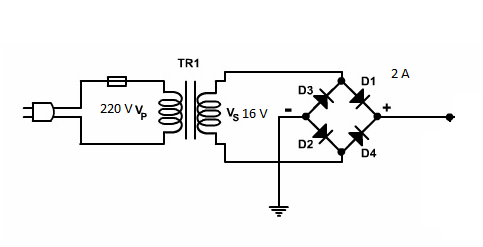
\includegraphics[scale=0.5]{figuras/circuitoretificadorcarregador}
	\caption{Circuito do tipo Retificador em ponte utilizado no carregador.}
	\label{img:circuitoretificadorcarregador}
\end{figure}

Materiais utilizados:
\begin{itemize}
\item 1 Transformador de 16Vac com capacidade de 2A da marca Hayama;
\item 4 Diodos 2A;
\item 1 chave liga desliga;
\item 1 cabo de força.
\end{itemize}

 \begin{figure}[H]
	\centering
	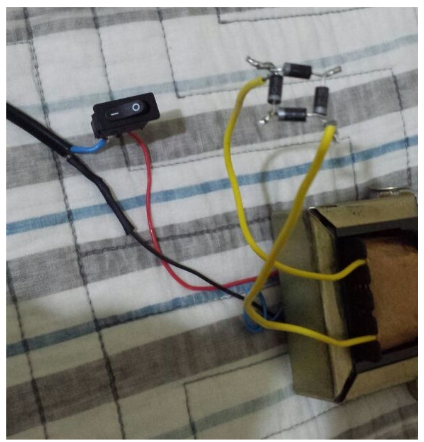
\includegraphics[scale=0.5]{figuras/fiosiotransformador}
	\caption{Fios de entrada e saída do transformador.}
	\label{img:fiosiotransformador}
\end{figure}

Em resumo, o sistema começa a funcionar a partir  do momento em que o cabo de força é conectado a tomada normal, a chave liga desliga é acionada para a passagem de corrente e a tensão é rebaixada pelo transformador, sendo retificada através da disposição de 4 diodos na saída de baixa tensão.
A tensão de 110V do não foi utilizada por conta de utilizarmos apenas as tomadas de entrada de 220V em Brasília, que por conta do transformador sofre uma queda para 13.13V como é possível ver na figura abaixo: 

 \begin{figure}[H]
	\centering
	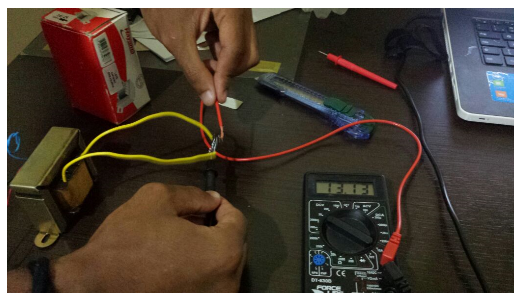
\includegraphics[scale=0.5]{figuras/medicaoafericaotensao}
	\caption{Medição para aferição da tensão de saída.}
	\label{img:medicaoafericaotensao}
\end{figure}

Observou-se que a tensão transformada, no lado de baixa, que deve ser entregue pelo carregador não foi de exatamente 16V. Essa queda de tensão pode ser explicada pelas perdas ocasionadas pelas resistências dos condutores bem como durante o processo de retificação em si.

 \begin{figure}[H]
	\centering
	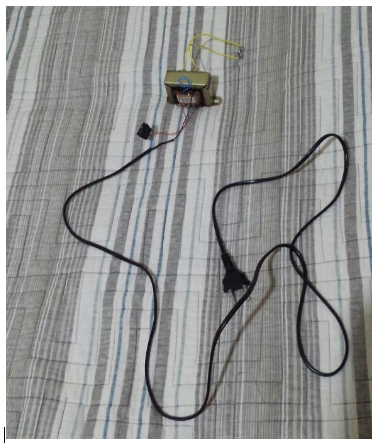
\includegraphics[scale=0.5]{figuras/carregadorsemplugmag}
	\caption{Carregador sem o plug magnético.}
	\label{img:carregadorsemplugmag}
\end{figure}

 \begin{figure}[H]
	\centering
	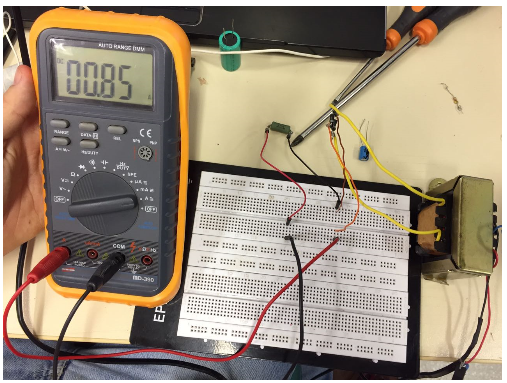
\includegraphics[scale=0.5]{figuras/testedecorrentecarregador}
	\caption{Teste de corrente.}
	\label{img:testedecorrentecarregador}
\end{figure}

Foi feito um teste para visualizar a corrente a ser entregue usando um resistor com potência de 5W, de acordo com a figura abaixo, obtém-se uma corrente de 0,85A em uma tensão de 13,3V. Se aumentar a potência do resistor é possível aumentar a corrente.


 \begin{figure}[H]
	\centering
	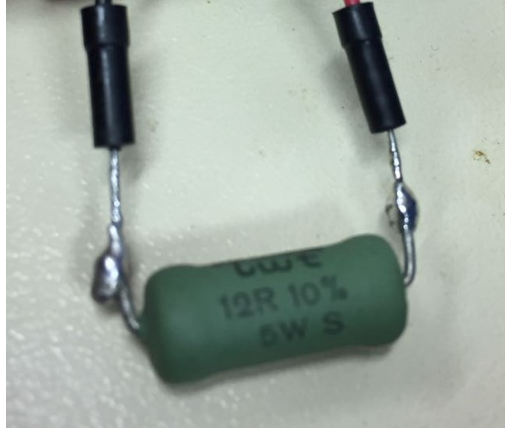
\includegraphics[scale=0.5]{figuras/resistorpotencia5w}
	\caption{Resistor com potência de 5W.}
	\label{img:resistorpotencia5w}
\end{figure}

Quanto ao conector com a carga a ser alimentada, no caso as baterias, escolheu-se que o mesmo seria do tipo plug magnético visando facilitar a conexão e honrar a proposta inicial do projeto de ser um dispositivo de funcionamento autônomo. O cabo de conexão está passando por testes e ajustes para poder ser acoplado à base do sistema já obtido a fim de disponibilizar mais uma solução viável para o suprimento de carga energética do sistema.
O plug magnético é formado por duas peças. A primeira é um pequeno conector que é acoplado na entrada do robô. A segunda é um pequeno adaptador no qual é conectado o cabo do carregador e que possui uma extremidade magnética que se encaixa de forma natural e fluida na outra ponta, iniciando na hora a recarga. Os cabos ainda não foram implementados na estrutura do plug.

 \begin{figure}[H]
	\centering
	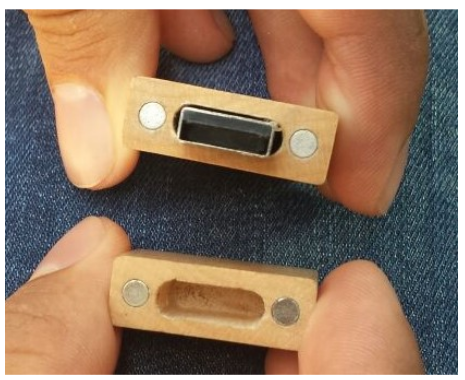
\includegraphics[scale=0.5]{figuras/peca1peca2}
	\caption{Peça 1 e Peça 2 Respectivamente.}
	\label{img:peca1peca2}
\end{figure}

 \begin{figure}[H]
	\centering
	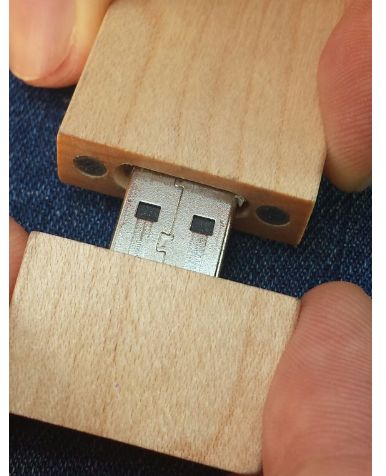
\includegraphics[scale=0.5]{figuras/interacaopolosmagneticos}
	\caption{Interação entre os pólos magnéticos.}
	\label{img:interacaopolosmagneticos}
\end{figure}

	% subsection carregador (end)
\subsection{Supercapacitores}
Supercapacitores vem sendo cada vez mais utilizados para o armazenamento de energia de curta duração, mesmo em situações onde pulsos intermitentes de alta energia são necessitados \cite{supercampos}.
Das aplicações usuais pode-se destacar a utilização em flashes fotográficos e veículos de transporte público, como trens e metrôs, onde a frenagem libera energia que é armazenada nos supercapacitores que, por sua vez, transferem essa energia ao motor durante a arrancada, gerando  mais potência nesses momentos [1].
Na tabela a seguir é um comparativo entre baterias e supercapacitores, também chamados de supercondensadores: 

\begin{table}[]
\centering
\caption{Bateria vs supercondensador.}
\label{tab:supervbat}
\begin{tabular}{|l|l|l|}
\hline
\multicolumn{1}{|l|}{\textbf{}}                                                                & \multicolumn{1}{l|}{\textbf{Bateria}} & \multicolumn{1}{l|}{\textbf{Supercondensador}} \\ \hline
\multicolumn{1}{|l|}{Tempo de carga}                                                           & \multicolumn{1}{l|}{1 a 5 horas}      & \multicolumn{1}{l|}{0,3 a 30 segundos}         \\ \hline
\multicolumn{1}{|l|}{Tempo de descarga}                                                        & \multicolumn{1}{l|}{0,3 a 3 horas}    & \multicolumn{1}{l|}{0,3 a 30 segundos}         \\ \hline
\multicolumn{1}{|l|}{\begin{tabular}[c]{@{}l@{}}Densidade de Energia\\ (Wh/kg)\end{tabular}}   & \multicolumn{1}{l|}{10 a 100}         & \multicolumn{1}{l|}{1 a 10}                    \\ \hline
\multicolumn{1}{|l|}{Cliclo de vida}                                                           & \multicolumn{1}{l|}{1000}             & \multicolumn{1}{l|}{\textgreater 500000}       \\ \hline
\multicolumn{1}{|l|}{\begin{tabular}[c]{@{}l@{}}Densidade de\\ Potência (W/kg)\end{tabular}}   & \multicolumn{1}{l|}{\textless 1000}   & \multicolumn{1}{l|}{\textless 10000}           \\ \hline
\multicolumn{1}{|l|}{\begin{tabular}[c]{@{}l@{}}Eficiência de carga\\ e descarga\end{tabular}} & \multicolumn{1}{l|}{0,7 a 0,85}       & \multicolumn{1}{l|}{0,85 a 0,98}               \\ \hline
\multicolumn{1}{|l|}{\begin{tabular}[c]{@{}l@{}}Temperatura de\\ operação\end{tabular}}                              & \multicolumn{1}{l|}{-20 a 100 oC}                          & \multicolumn{1}{l|}{-40 a 65 oC}                                   
\end{tabular}
\end{table}

Analisando a tabela nota-se claramente que supercapacitores são melhor utilizados quando sua aplicação se da em curto espaços de tempo. 
A tensão dos supercapacitores diminui, com a descarga, de forma linear, o que acarreta em um não aproveitamento do espectro energético do dispositivo \cite{supersantos}.
Ainda temos que supercapacitores perdem maior quantidade de energia com a auto descarga \cite{supersantos}.
O projeto em questão necessita de um tempo longo (quando comparado ao tempo de descarga de um supercapacitor) de uso, além disso, os outros fatores supracitados influenciam de forma desfavorável ao supercapacitor, acarretando na não escolha desse método de armazenamento de energia.
% section alimentação (end)
